The following sections will discuss the results of our baseline experiments, further ideas for the project, and real-world applications of the project.

\subsection{Baseline Experiments}\label{subsec:baseline-results}
We did an exemplary training for 10 epochs on a subset of ImageNet to see if it converges.
The training subset contained 100,000 images with 100 samples per class, while the test subset contained 10,000 samples, 10 per class.
We used the PyTorch implementation of the Adam optimizer with a learning rate of 0.001 with a batch size of 128.
This resulted in roughly 780 optimization steps per epoch.
We chose to use 2 latent channels per latent variable using the 32 bit float of pytorch.

\begin{figure}
    \centering
    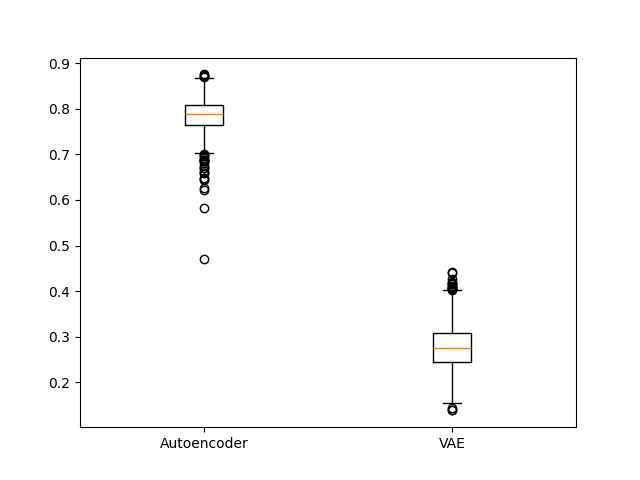
\includegraphics[width=0.4\textwidth]{../../sample_images/evaluation/boxplot_ae_and_vae}
    \caption{Boxplots of per class average SSIM on test data}
    \label{fig:boxplots}
\end{figure}

\begin{figure}
    \centering
    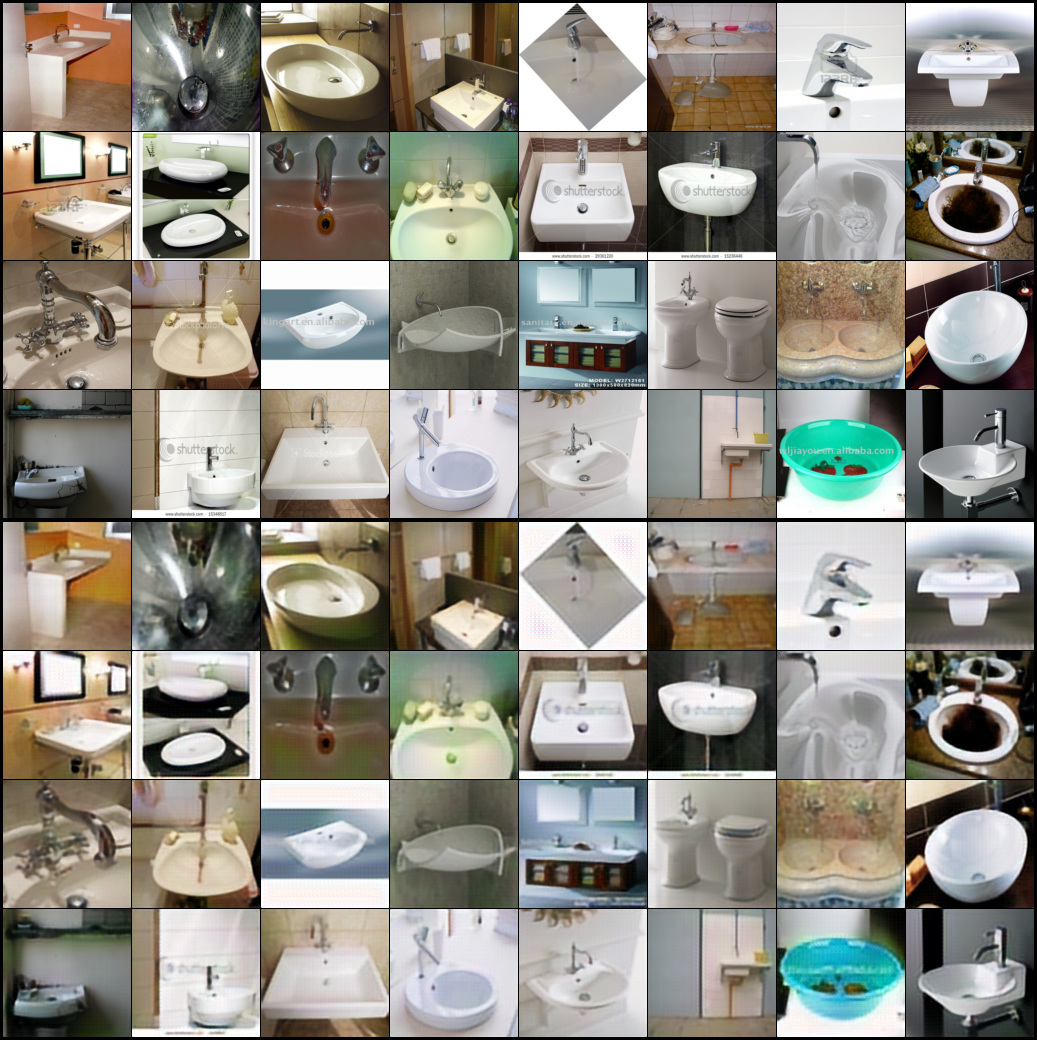
\includegraphics[width=0.4\textwidth]{../../sample_images/evaluation/MAX_AE_IDX_896}
    \caption{Best performing class (896) of Autoencoder with SSIM of 0.88}
    \label{fig:imnet_best_perf_ae}
\end{figure}

\begin{figure}
    \centering
    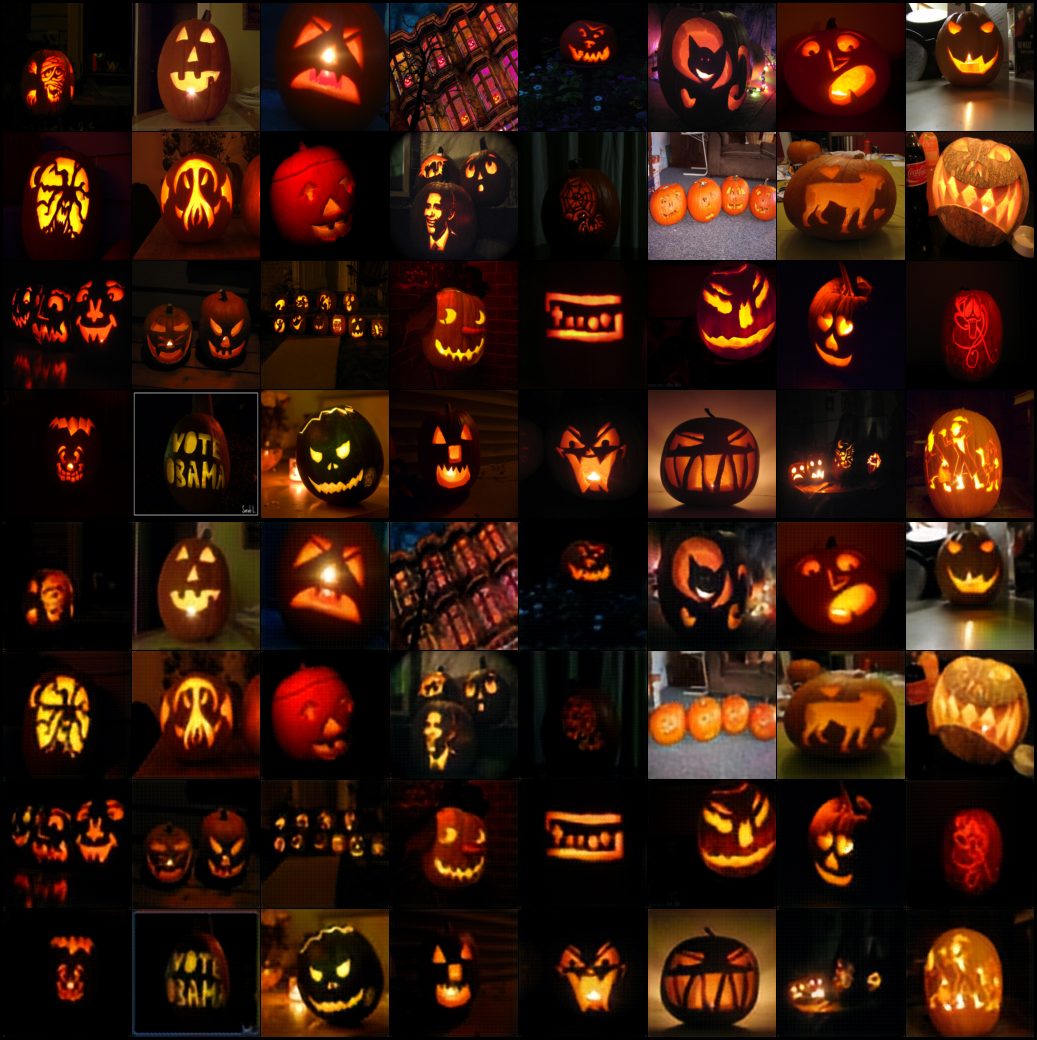
\includegraphics[width=0.4\textwidth]{../../sample_images/evaluation/MIN_AE_IDX_607}
    \caption{Worst performing class (607) of autoencoder with SSIM of 0.47}
    \label{fig:imnet_worst_perf_ae}
\end{figure}

\begin{figure}
    \centering
    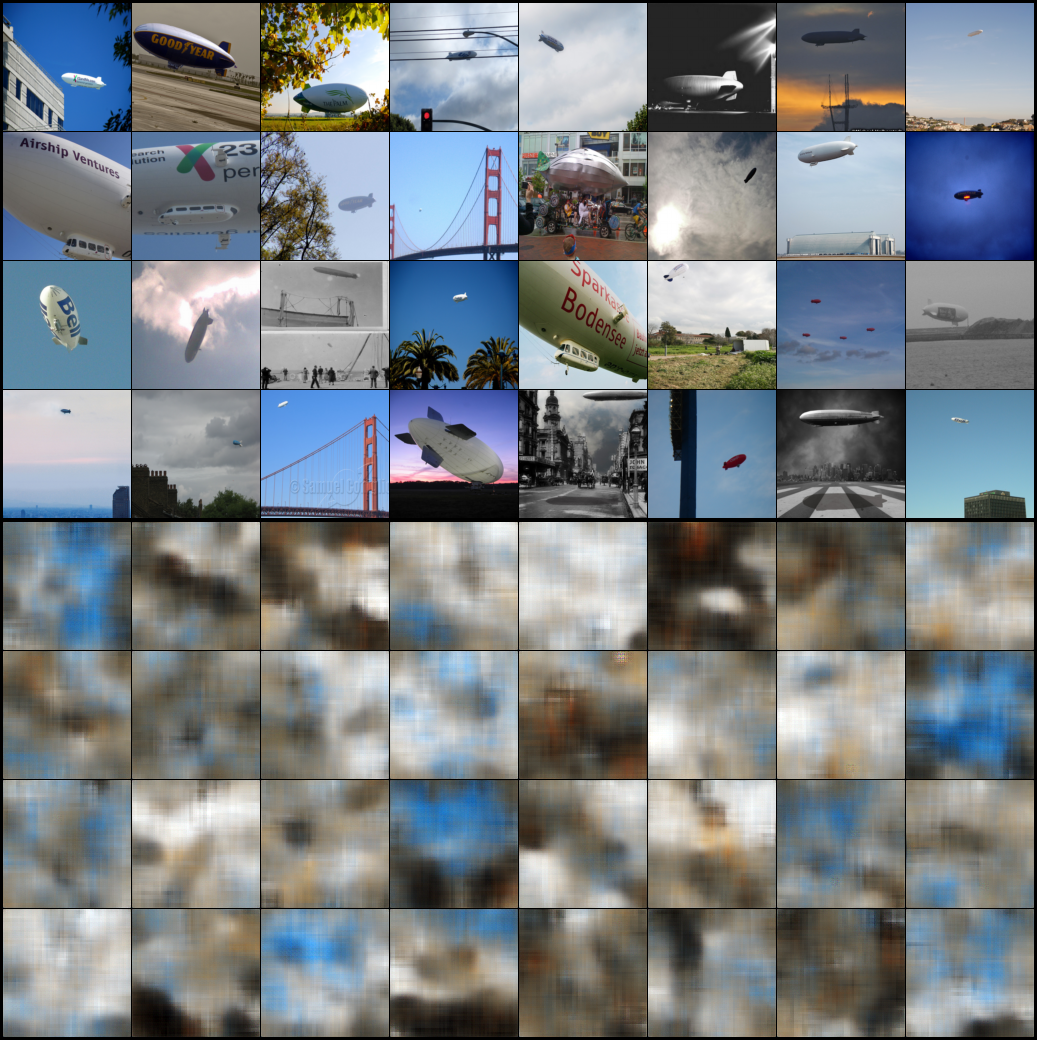
\includegraphics[width=0.4\textwidth]{../../sample_images/evaluation/MAX_VAE_IDX_405}
    \caption{Best performing class (405) of VAE with SSIM 0.44}
    \label{fig:imnet_best_perf2_vae}
\end{figure}

\begin{figure}
    \centering
    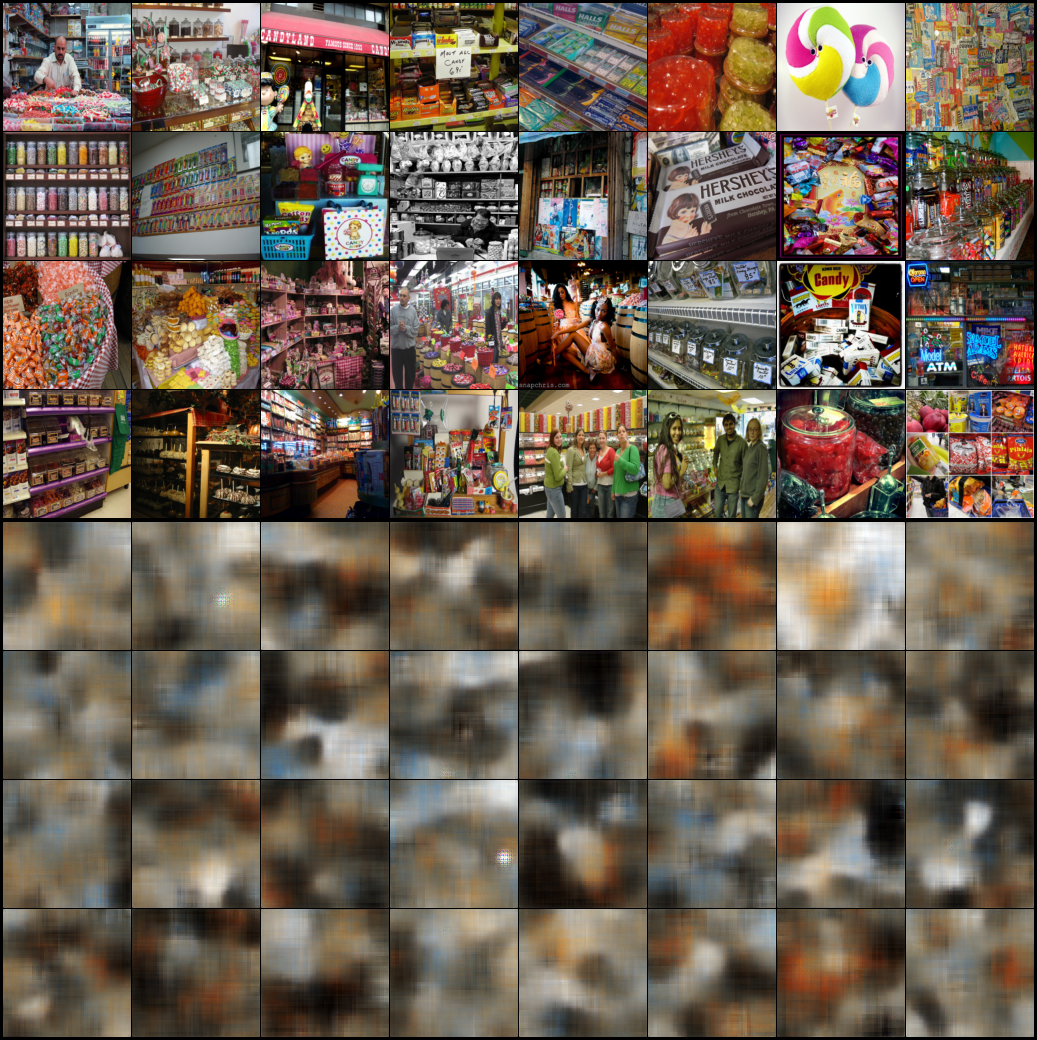
\includegraphics[width=0.4\textwidth]{../../sample_images/evaluation/MIN_VAE_IDX_509}
    \caption{Worst performing class (509) of VAE with SSIM 0.19}
    \label{fig:imnet_worst_perf2_vae}
\end{figure}

\subsubsection{JPEG}\label{subsubsec:autoencoder}
To compare the compression ability of our baseline methods to JPEG compression, we first had to identify the quality with which JPEG compresses images to approximately 4 bits per pixel.
We found that 4 bits per pixel where achieved even when using JPEG compression with a quality parameter of 100.
This shows that neural image compression with the baseline methods we implemented merely exist for research purposes and do not pose an actual benefit when the goal would be to compress images.


\subsubsection{Autoencoder}\label{subsubsec:autoencoder}
When feeding in $3 \times 128 \times 128$ ImageNet images, our latents are of size $\mathbb{R}^{2\times 32 \times 32}$.
From initially $24\text{ bits/pixel}$, the images are compressed down to $4\text{ bits/pixel}$.
We therefore reach a compression rate of 1:6.

We were able to show that our implementation of an \ac{ae} is able to reconstruct images from the ImageNet dataset
passing a first human look.
The average of the SSIM of the test data is $\tilde0.78$ as can be seen in figure~\cite{citationNeeded}.

\subsubsection{VAE}\label{subsubsec:vae_training}
When using the same latent size as for the \ac{ae}, the \ac{vae} was not able to obtain reconstructions
passing a first visual check.
The numeric metrics were also very low.
The decoder produced samples that were always very similar, indicating that it suffered from posterior collapse.
We plan to revisit our implementation later and analyze if we can make it more useful as a baseline.

\subsubsection{Class Differences}\label{subsubsec:class-differences}
Going deeper into analyzing the performance of our baseline methods, we evaluated their SSIM per class.
Hoping to gain insights to potentially improve robustness of future implementations, MEHR GELABER KP.
The distribution of MSSIM of the images of each class for both VAE and Autoencoder are shown in figure~\cite{citationNeeded}.

\subsection{Dataset}\label{subsec:dataset}

\subsubsection{Realworld Application}
\ac{cifar} and ImageNet have been foundational datasets for over a decade and a half.
Their primary use-case has shifted from being cutting-edge datasets for training state-of-the-art models like the
work from~\cite{AlexNet}, to serving as a base for experiments and benchmarks.

Nowadays, state-of-the-art generative models rely on much larger datasets, often containing billions of samples.
A notable example is LAION-5B~\cite{laion5b} which was used to train the Stable Diffusion model introduced by~
\cite{stable_diff}.

Throughout the same paper ImageNets continuing relevancy can be observed, as it is used to train and evaluate
experimental models.
Its still substantial capacity allows for the generalization of good performance to larger and more diverse datasets.
Additionally, inception based metrics like \ac{fid} are also calculated using ImageNet.

Similar trends can be observed with CIFAR-10; however, its low resolution restricts its applicability for
benchmarking contemporary image generation approaches.

\subsubsection{Suitability}
While we still intend to work with CIFAR-10 for comparison and fast prototyping, its lower capacity makes it less
promising to us.

Despite the assessment that ImageNet is comparably smaller than current datasets used for commercially used models, it is
still a big and diverse dataset.
This poses the biggest advantage, but also the biggest challenge with this dataset for us.

The challenge comes in the form of heterogeneous shapes and properties of individual classes and their distributions.
Its size forces us to rely heavily on statistical analysis, as sample inspection has only limited applicability at
this scale.

On the other hand, the size and diversity of the data is of course a huge advantage for training the models.
The models will be able to learn a wide range of features and patterns, and to generalize it to unseen data.

The results from our initial training runs, using only a small subset of the training data, demonstrate promising
outcomes.
Judging by the plots in figure ~\cite{citationNeeded}, the model has neither converged on test nor the training data.
We therefore expect some headroom for training the model on the full dataset until convergence, further improving
performance.

Sampling functionality has not yet been implemented; however, due to its still widespread use for experimental
models we are certain that the dataset is sufficient for training our generative models.
Especially due to its comparably lower size to modern datasets, we do not anticipate achieving the level of visual
fidelity demonstrated by state-of-the-art techniques.

\subsection{A prospect on further Experiments}\label{subsec:further-ideas}
We utilize the structural similarity index as a metric for image similarity to evaluate the reconstruction quality
of our models~\ref{subsec:compression}.
For comparison to the paper, we still use \ac{mse} loss for training our \ac{ae}.
Though, as discussed in~\ref{subsec:compression}, \ac{mse} might not be the optimal metric in terms of human perception.

\ac{ssim} is a metric for precisely this purpose, so we think our models might benifit from using it as a loss
function instead of \ac{mse}.
In ~\cite{ssim_as_loss}, it is shown that using a loss function trageted to human perception can improve the quality
of convolutional neural networks for image reconstruction, in particular using \ac{ssim}.

\subsection{Working Title: Final words}\label{subsec:final-words}
Image reconstruction as well as image generation are two relatively well researched topics.
Presumably, because of their wide range of applications.
While the most prominent methods, i.e. \ac{ae} and \ac{vae}, are two simple yet powerful models, they still have
their limitations.

\ac{ae} are powerful reconstructors, but they are not able to generate new images, because of their deterministic
nature and their discrete latent representation.

\ac{vae} can sample in the latent space and generate new images by virtue of their stochastic properties.
Yet, you sometime favour a discrete latent over latent distributions, because of their simplicity, interpretability
and compatibility with other modalities ~\cite{vqvae}.

\ac{vq} is an attempt to fill that gap.
It enables to reconstruct images, generate new samples while having a discrete latent representation.

\vskip 1em
\textbf{A Note on Overfitting:}
Overfitting refers to the phenomenon where a model starts to memorize the training data instead of learning useful
features, in turn not generalizing well to unseen data.

While theoretically, this may very well be an issue with \ac{ae} and \ac{vae}, we have not experienced this happening
yet with either when training with adequate training-set sizes.a
This is likely due to the large dataset sizes we use and the inductive bias of the convolution operation~
\cite{citationNeeded}.